\section{A Real Time Spectrum Analyser Using Least Mean Square}

\begin{enumerate}[label=\alph*), leftmargin=*]

%% a)
\item
%

Let the $L_{2}$-norm of the prediction error being the objective function $\mathcal{J}$:

\begin{equation}
    \mathcal{J}(\vw) = \| \vy - \hat{\vy} \|^{2} = \| \vy - \mathbf{F} \vw \|^{2} = (\vy - \mathbf{F} \vw)^{H} (\vy - \mathbf{F} \vw)
\label{eq:J_OLS}
\end{equation}

In order to minimise the objective function $\mathcal{J}$ with respect to the parameters (weights) $\vw$, the first order condition is:

\begin{equation}
    \frac{\partial \mathcal{J}(\vw)}{\partial \vw} \bigg\vert_{\vw=\vw_{*}}  = 0
\end{equation}

Substituting from (\ref{eq:J_OLS}):

\begin{align}
    \frac{\partial}{\partial \vw} \bigg( \vy^{H} \vy - \vy^{H} \mathbf{F} \vw - \vw^{H} \mathbf{F}^{H} \vy + \vw^{H} \mathbf{F}^{H} \mathbf{F} \vw \bigg) \bigg\vert_{\vw=\vw_{*}}  &= 0 \\
    0 - \mathbf{F}^{H} \vy - \mathbf{F}^{H} \vy + 2 \mathbf{F}^{H} \mathbf{F} \vw_{*} &= 0
\end{align}

Assuming that $\mathbf{F}^{H} \mathbf{F}$ is invertible (\textbf{semi}-positive as covariance matrix), we solve for $\vw_{*}$, concluding the proof:

\begin{equation}
    \vw_{*} = \bigg( \mathbf{F}^{H} \mathbf{F} \bigg)^{-1} \mathbf{F}^{H} \vy
\label{proof:OLS}
\end{equation}

The Inverse Discrete Fourier Transform (IDFT) of a signal $x(n)$ is given by:

\begin{align}
    \hat{x}(n)  &= \frac{1}{\sqrt{N}} \sum_{k=0}^{N-1} X(k) e^{j \frac{2\pi}{N} n k}
                 = \frac{1}{\sqrt{N}} \sum_{k=0}^{N-1} X(k) F_{N}^{nk}
\end{align}

where $F_{N} = e^{j \frac{2\pi}{N}}$. If we define:

\begin{equation}
    \renewcommand\arraystretch{1.5}
    \vf_{n}^{H} = \frac{1}{\sqrt{N}}
    \begin{bmatrix}
        1, & F_{N}^{n}, & F_{N}^{2n}, & \ldots, & F_{N}^{n(N-1)}
    \end{bmatrix}
\end{equation}

Arranging the sample estimates in a vector, we obtain:

\begin{equation}
    \renewcommand\arraystretch{1.5}
    \hat{\vx} =
    \begin{bmatrix}
        \hat{x}(0) \\ \hat{x}(1) \\ \vdots \\ \hat{x}(N-1)
    \end{bmatrix}
    =
    \begin{bmatrix}
        \vf_{0}^{H} \mathbf{X} \\ \vf_{1}^{H} \mathbf{X} \\ \vdots \\ \vf_{N-1}^{H} \mathbf{X}
    \end{bmatrix}
    =
    \mathbf{F} \mathbf{X}
\label{eq:DFT_OLS}
\end{equation}

where:

\begin{equation}
    \renewcommand\arraystretch{1.5}
    \mathbf{F} =
    \begin{bmatrix}
        \vf_{0}^{H} \\ \vf_{1}^{H} \\ \vdots \\ \vf_{N-1}^{H}
    \end{bmatrix}
    = \frac{1}{\sqrt{N}}
    \begin{bmatrix}
        1 & 1 & 1 & \cdots & 1 \\
        1 & F_{N} & F_{N}^{2} & \cdots & F_{N}^{N-1} \\
        \vdots & \vdots & \vdots & \ddots & \vdots \\
        1 & F_{N}^{N-1} & F_{N}^{2(N-1)} & \cdots & F_{N}^{(N-1)^{2}} \\
    \end{bmatrix}
\end{equation}

Hence from (\ref{eq:DFT_OLS}), we conclude that IDFT is a linear transformation, where $\mathbf{F}$ the transformation matrix comprises of N harmonically related sinusoids,
with mutually orthonormal columns\footnote{Note that the $\frac{1}{\sqrt{N}}$ term is introduce to deal with unit-length columns.}. Then the Fourier coefficients, $\mathbf{X}$, are given by (\ref{proof:OLS}):

\begin{equation}
    \mathbf{X} = \bigg( \mathbf{F}^{H} \mathbf{F} \bigg)^{-1} \mathbf{F}^{H} \hat{\vx} = \mathbf{F}^{H} \hat{\vx}
\label{proof:DFT_as_OLS}
\end{equation}

where the fact that $\mathbf{F}$ is unitary is used\footnote{See Problem \& Answer Sets for the proof.}.
Therefore, since (\ref{proof:OLS}) is the optimal least mean squares solution, minimising the squared error and the Fourier coefficients, $\vw$, follow (\ref{proof:OLS}),
then Inverse Discrete Fourier Transform, $\hat{x}(n)$, is a linear approximation of the original signal $x(n)$, minimising the squared error:

\begin{equation}
    \underset{\mathbf{X}}{min} \| \vx - \hat{\vx} \|^{2}
\end{equation}

% The Discrete Fourier Transform (DFT) of a signal $x(n)$ is given by:

% \begin{align}
%     X(k)    &= \frac{1}{\sqrt{N}} \sum_{n=0}^{N-1} x(n) e^{-j \frac{2\pi}{N} n k}
%              = \frac{1}{\sqrt{N}} \sum_{n=0}^{N-1} x(n) W_{N}^{nk}
% \end{align}

% where $W_{N} = e^{-j \frac{2\pi}{N}}$. If we define:

% \begin{equation}
%     \renewcommand\arraystretch{1.5}
%     \vw_{k}^{H} = \frac{1}{\sqrt{N}}
%     \begin{bmatrix}
%         1, & W_{N}^{k}, & W_{N}^{2k}, & \ldots, & W_{N}^{k(N-1)}
%     \end{bmatrix}
% \end{equation}

% Arranging the DFT coefficients in a vector, we obtain:

% \begin{equation}
%     \renewcommand\arraystretch{1.5}
%     \mathbf{X} =
%     \begin{bmatrix}
%         X(0) \\ X(1) \\ \vdots \\ X(N-1)
%     \end{bmatrix}
%     =
%     \begin{bmatrix}
%         \vw_{0}^{H} \vx \\ \vw_{1}^{H} \vx \\ \vdots \\ \vw_{N-1}^{H} \vx
%     \end{bmatrix}
%     =
%     \mathbf{W} \vx
% \end{equation}

% where:

% \begin{equation}
%     \renewcommand\arraystretch{1.5}
%     \mathbf{W} =
%     \begin{bmatrix}
%         \vw_{0}^{H} \\ \vw_{1}^{H} \\ \vdots \\ \vw_{N-1}^{H}
%     \end{bmatrix}
%     = \frac{1}{\sqrt{N}}
%     \begin{bmatrix}
%         1 & 1 & 1 & \cdots & 1 \\
%         1 & W_{N} & W_{N}^{2} & \cdots & W_{N}^{N-1} \\
%         \vdots & \vdots & \vdots & \ddots & \vdots \\
%         1 & W_{N}^{N-1} & W_{N}^{2(N-1)} & \cdots & W_{N}^{(N-1)^{2}} \\
%     \end{bmatrix}
% \end{equation}




% The Fourier estimation of a signal $x(n)$, or equivalently its Inverse Discrete Fourier Transform (IDFT), satisfy:

% \begin{align}
%     \hat{x}(n)  &= \frac{1}{\sqrt{N}} \sum_{k=0}^{N-1} X(k) e^{j 2\pi k n / N} \\
%                 &= \frac{1}{\sqrt{N}} \bigg[ X(0) + X(1) e^{j 2\pi n / N} + X(2) e^{(j 2\pi n / N) 2} + \ldots + X(N-1) e^{(j 2\pi n / N) (N-1)} \bigg]
% \end{align}

% Rewriting the equation above in matrix form:

% \begin{align}
%     \renewcommand\arraystretch{1.5}
%     \begin{bmatrix}
%         \hat{x}(0) \\ \hat{x}(1) \\ \vdots \\ \hat{x}(N-1)
%     \end{bmatrix}
%     = \frac{1}{\sqrt{N}}
%     \begin{bmatrix}
%         1 & 1 & \cdots & 1 \\
%         1 & e^{j \frac{2\pi}{N}(1)(1)} & \cdots & e^{j \frac{2\pi}{N}(1)(N-1)} \\
%         \vdots & \vdots & \ddots & \vdots \\
%         1 & e^{j \frac{2\pi}{N}(1)(N-1)} & \cdots & e^{j \frac{2\pi}{N}(N-1)(N-1)}
%     \end{bmatrix}
%     \begin{bmatrix}
%         X(0) \\ X(1) \\ \vdots \\ X(N-1)
%     \end{bmatrix}
% \end{align}

% Letting $a = e^{j\frac{2\pi}{N}}$, we notice a pattern, such that:

% \begin{align}
%     \renewcommand\arraystretch{1.5}
%     \underbrace{
%         \begin{bmatrix}
%             \hat{x}(0) \\ \hat{x}(1) \\ \vdots \\ \hat{x}(N-1)
%         \end{bmatrix}
%     }_{\hat{\vx}}
%     = \frac{1}{\sqrt{N}}
%     \underbrace{
%         \begin{bmatrix}
%             1 & 1 & \cdots & 1 \\
%             1 & a & \cdots & a^{(N-1)} \\
%             \vdots & \vdots & \ddots & \vdots \\
%             1 & a^{(N-1)} & \cdots & a^{(N-1)(N-1)}
%         \end{bmatrix}
%     }_{\mathbf{F}}
%     \underbrace{
%         \begin{bmatrix}
%             X(0) \\ X(1) \\ \vdots \\ X(N-1)
%         \end{bmatrix}
%     }_{\vw}
% \end{align}

% We conclude that the IDFT is a linear transformation, where $\mathbf{F}$ the transformation matrix comprises of N harmonically related sinusoids, with mutually orthonormal columns\footnote{Note that the
% $\frac{1}{\sqrt{N}}$ term is introduce to deal with unit-length columns.}. Then the Fourier coefficients, $\vw$, are given by (\ref{proof:OLS}):

% \begin{equation}
%     \vw = \bigg( \mathbf{F}^{H} \mathbf{F} \bigg)^{-1} \mathbf{F}^{H} \vx = \mathbf{F}^{H} \vx
% \end{equation}

% where the fact that $\mathbf{F}$ is unitary is used\footnote{See Problem \& Answer Sets for the proof.}.

% Hence, since (\ref{proof:OLS}) is the optimal least mean squares solution, minimising the squared error and the Fourier coefficients, $\vw$, follow (\ref{proof:OLS}),
% then Inverse Discrete Fourier Transform, $\hat{x}(n)$, is a linear approximation of the original signal $x(n)$, minimising the squared error:

% \begin{equation}
%     \underset{\vw}{min} \| \vx - \hat{\vx} \|^{2}
% \end{equation}

%% b)
\item
%

According to equation (\ref{proof:DFT_as_OLS}), the Fourier coefficients, $\mathbf{X}$, are a linear combination of the columns of the transformation matrix $\mathbf{F}$, whose columns are orthonormal:

\begin{equation}
    \vf_{k}^{H} \vf_{l} = \frac{1}{N} \sum_{k=0}^{N-1} e^{j \frac{2\pi}{N} (k-l)} = \left\{
    \begin{array}{ll}
      1 & \text{if } k=l\\
      0 & \text{otherwise}
\end{array} \right.
\end{equation}

Therefore DFT operation can be seen as a projection of a vector, $\vx$, in time domain to the $\mathbf{F}$ matrix subspace, spanned by their orthonormal columns,
representing $N$ harmonically related sinusoids, wnere each sinusoid is a multiple of the frequency $\frac{f_{s}}{N}$, with $f_{s}$ the sampling frequency.

%% c)
\item
%

The $K$-points DFT-CLMS method is applied to the frequency modulated (FM) non-stationary signal, $f(n)$. Figure \ref{fig:4_3_c_1} illustrates the time-frequency diagram obtained.
The algorithm adapts perfectly to the behaviour of the frequency signal, $f(n)$, for $n < 500$, where the frequency is constant over time, while for larger values we notice
that the trends (both linear and quadratic) are generally captured. Surprisingly though, once a strong frequency component is picked up by the DFT-CLMS filter, this component is not updated,
hence the diagram has Fourier coefficients superimposed over time. CLMS is a gradient algorithm, which updates weights (DFT coefficients)
towards the mean squared error descent direction. The coefficients are not block-based calculated, but in an adaptive manner, hence error back-propagation is slow, causing this
lasting effect. Moreover, the $K$-points DFT-CLMS filter has $K$ dimensional weights, where $K=2048$, thus the curse of dimensionality prevents error gradients to propagate back and update the weights.

\begin{figure}[h]
    \centering
    \begin{subfigure}{0.49\textwidth}
        \centering
        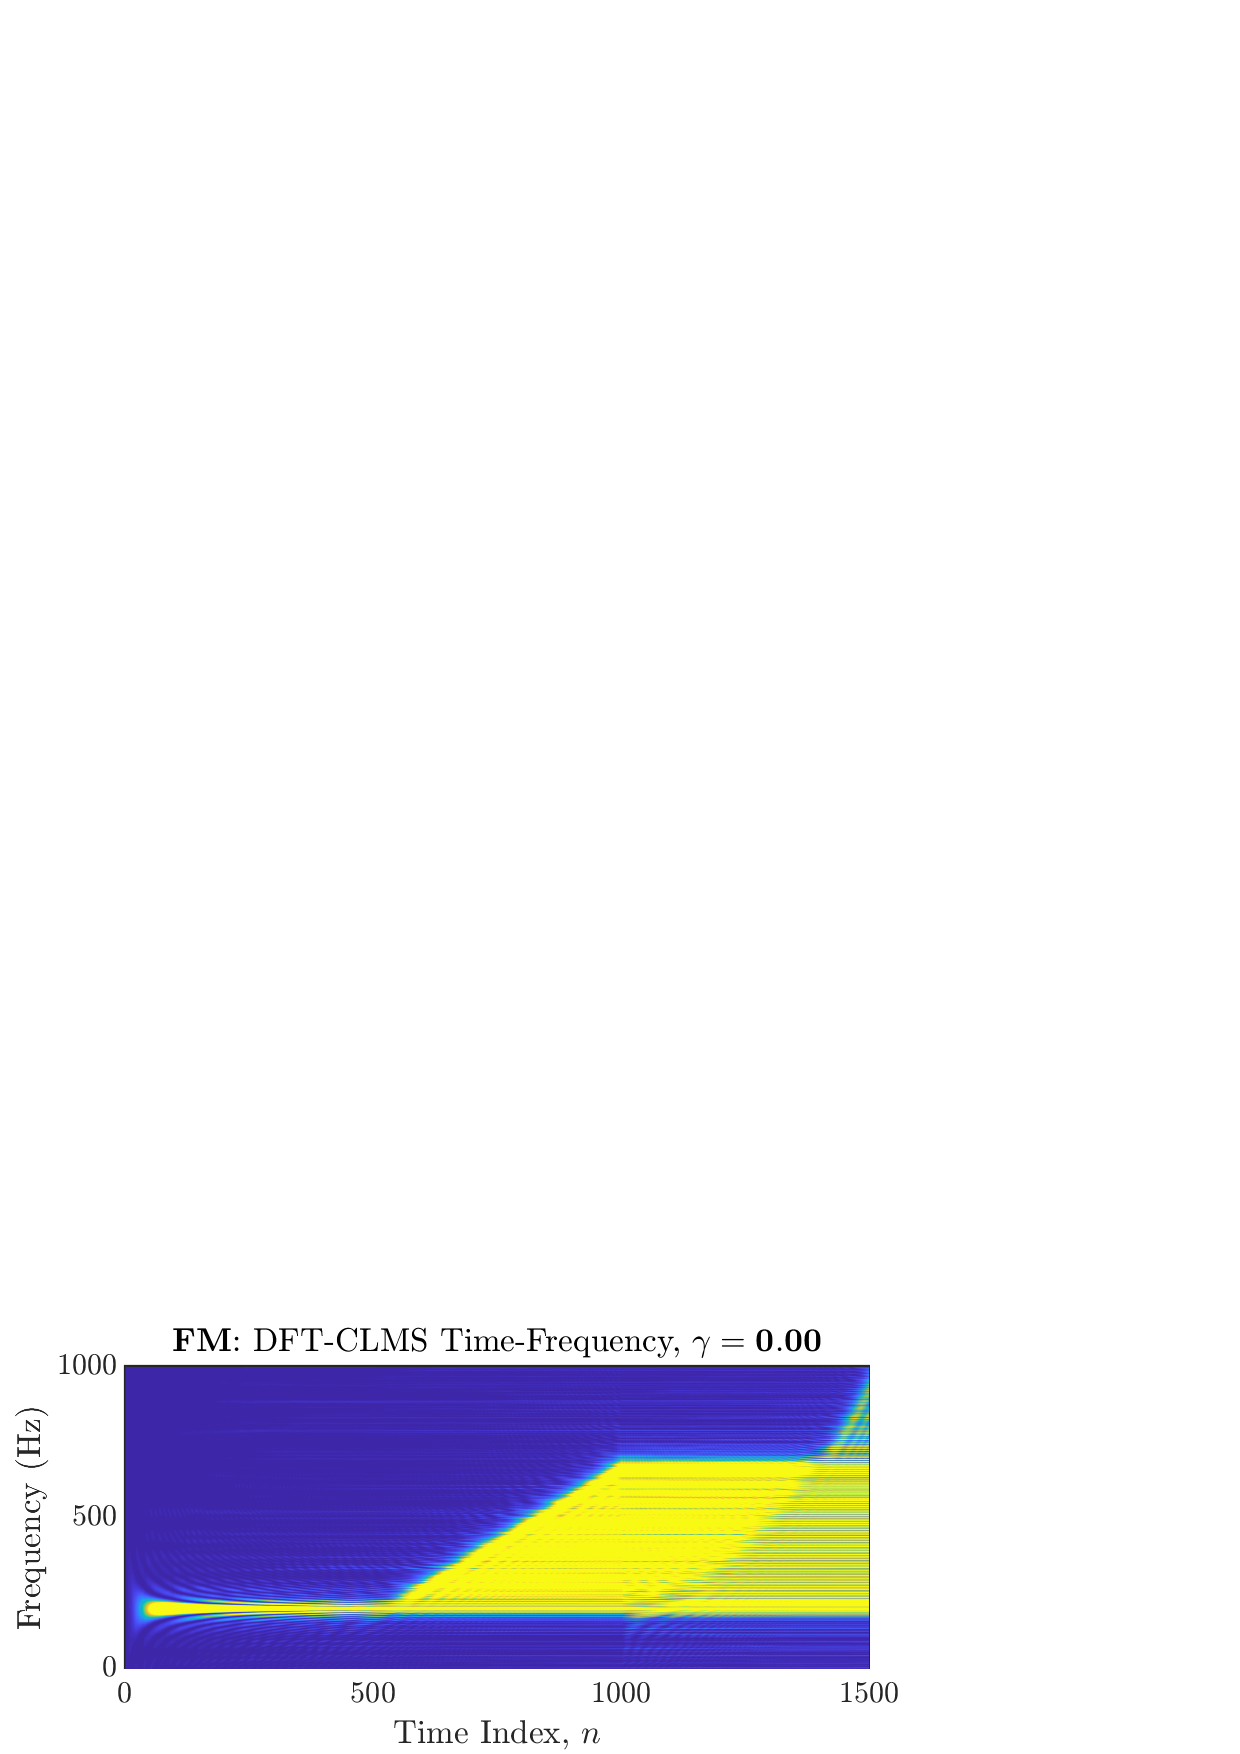
\includegraphics[height=1.5in]{{report/widely-linear-filtering-and-adaptive-spectrum-estimation/a-real-time-spectrum-analyser-using-least-mean-square/assets/c/dft_clms-gamma_0.00}.pdf}
    \end{subfigure}
    \caption{FM: DFT-CLMS time-frequency plot with $\gamma = 0$ (unbiased).}
    \label{fig:4_3_c_1}
\end{figure}

Regularisation, such as adding a leakage coefficient $\gamma$, similar to the Leaky LMS variant, enables accurate time-frequency modelling, as shown in figure \ref{fig:4_3_c_2}.
This is achieved thanks to the forget mechanism that the Leaky CLMS algorithm provides:

\begin{equation}
    \vw(n+1) = (1 -\gamma \mu) \vw(n) + \mu e^{*}(n) \vx(n)    
\end{equation}

where the greater $\gamma$ values allow to ignore, forget previous timestep's weights $\vw(n)$.

Note that for very small values of the leakage coefficient (i.e $\gamma = 0.01$) the Fourier coefficient superimposing effect is still visible.
However, larger values of $\gamma$ (i.e $\gamma = 0.05, 0.1$) introduce some bias, but obtain correct modelling. Finally, bias for larger values of $\gamma$ (i.e $\gamma \geq 0.5$) lead to inaccurate results.

\begin{figure}[h]
    \centering
    \begin{subfigure}{0.49\textwidth}
        \centering
        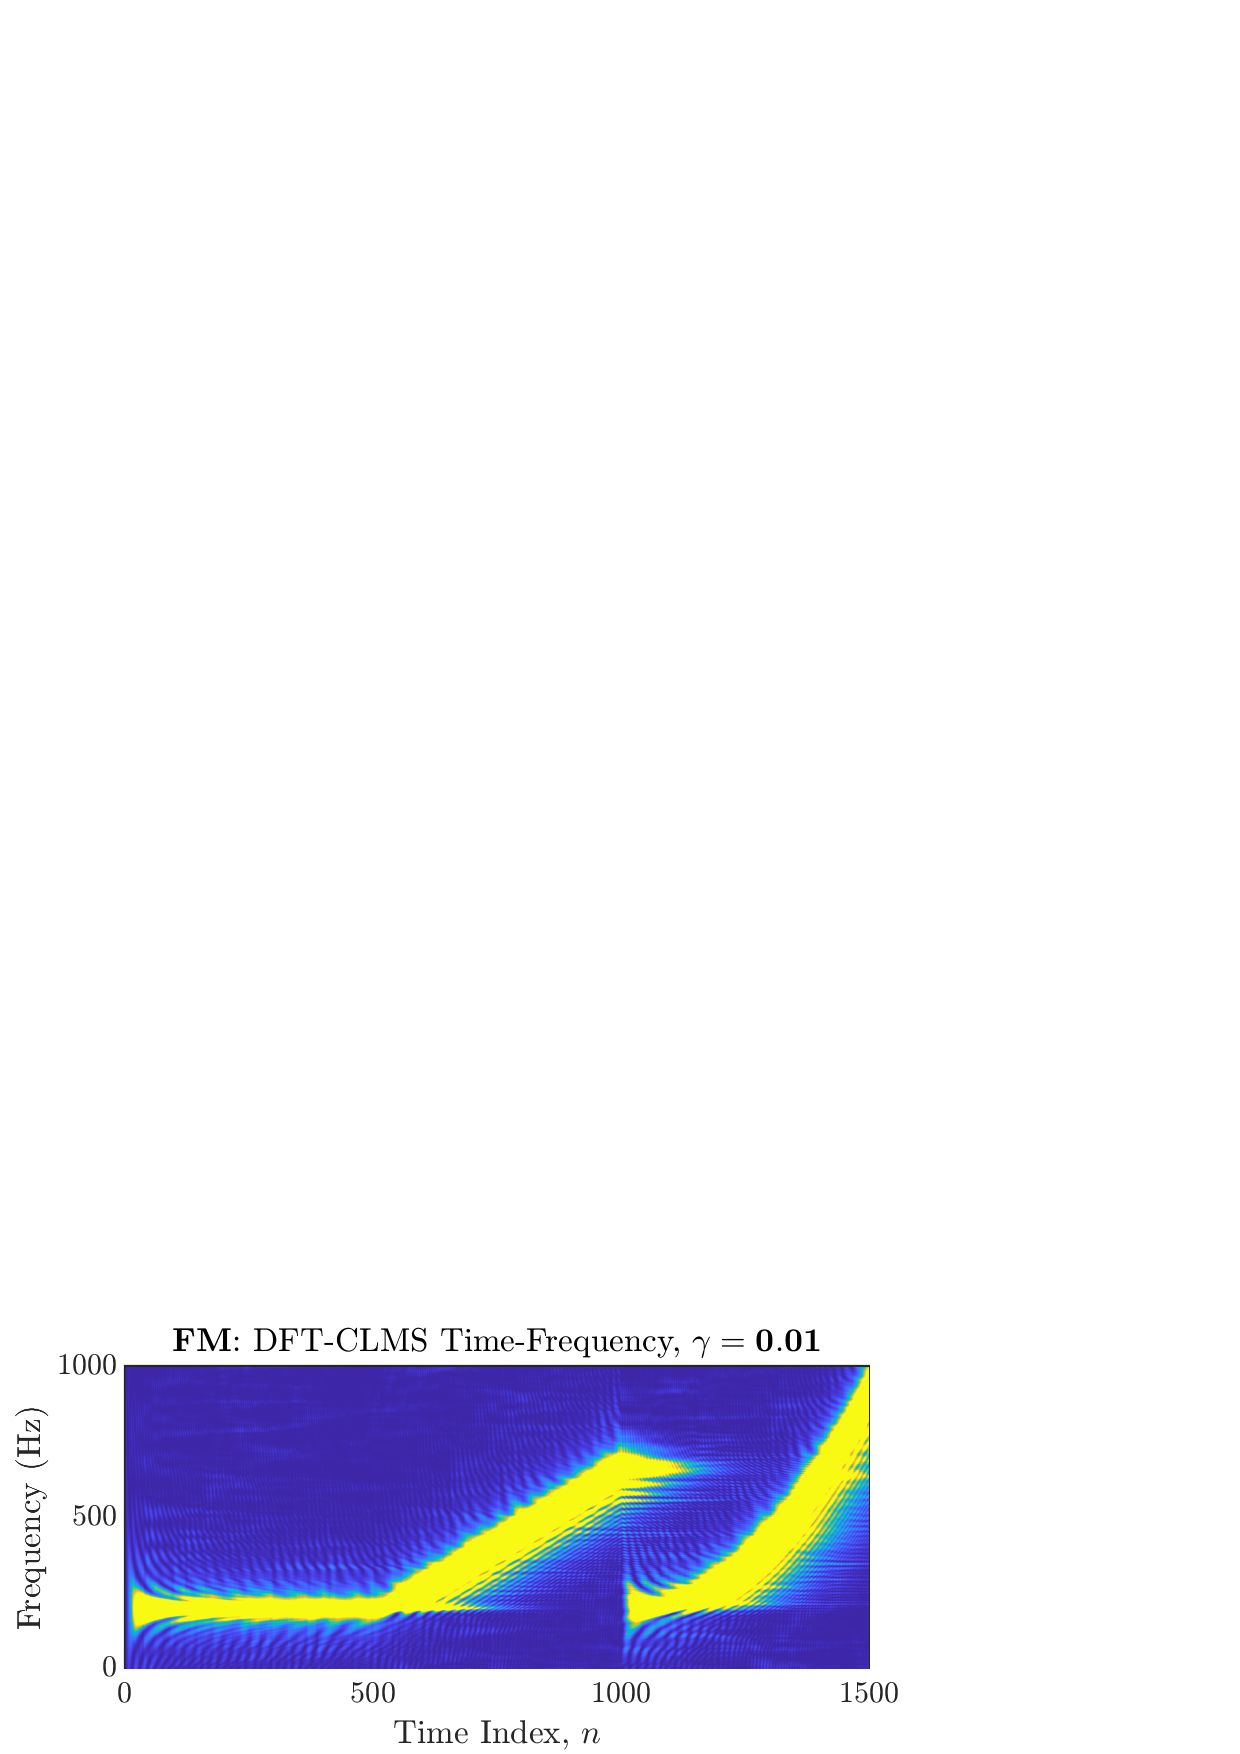
\includegraphics[height=1.5in]{{report/widely-linear-filtering-and-adaptive-spectrum-estimation/a-real-time-spectrum-analyser-using-least-mean-square/assets/c/dft_clms-gamma_0.01}.pdf}
    \end{subfigure}
    ~
    \begin{subfigure}{0.49\textwidth}
        \centering
        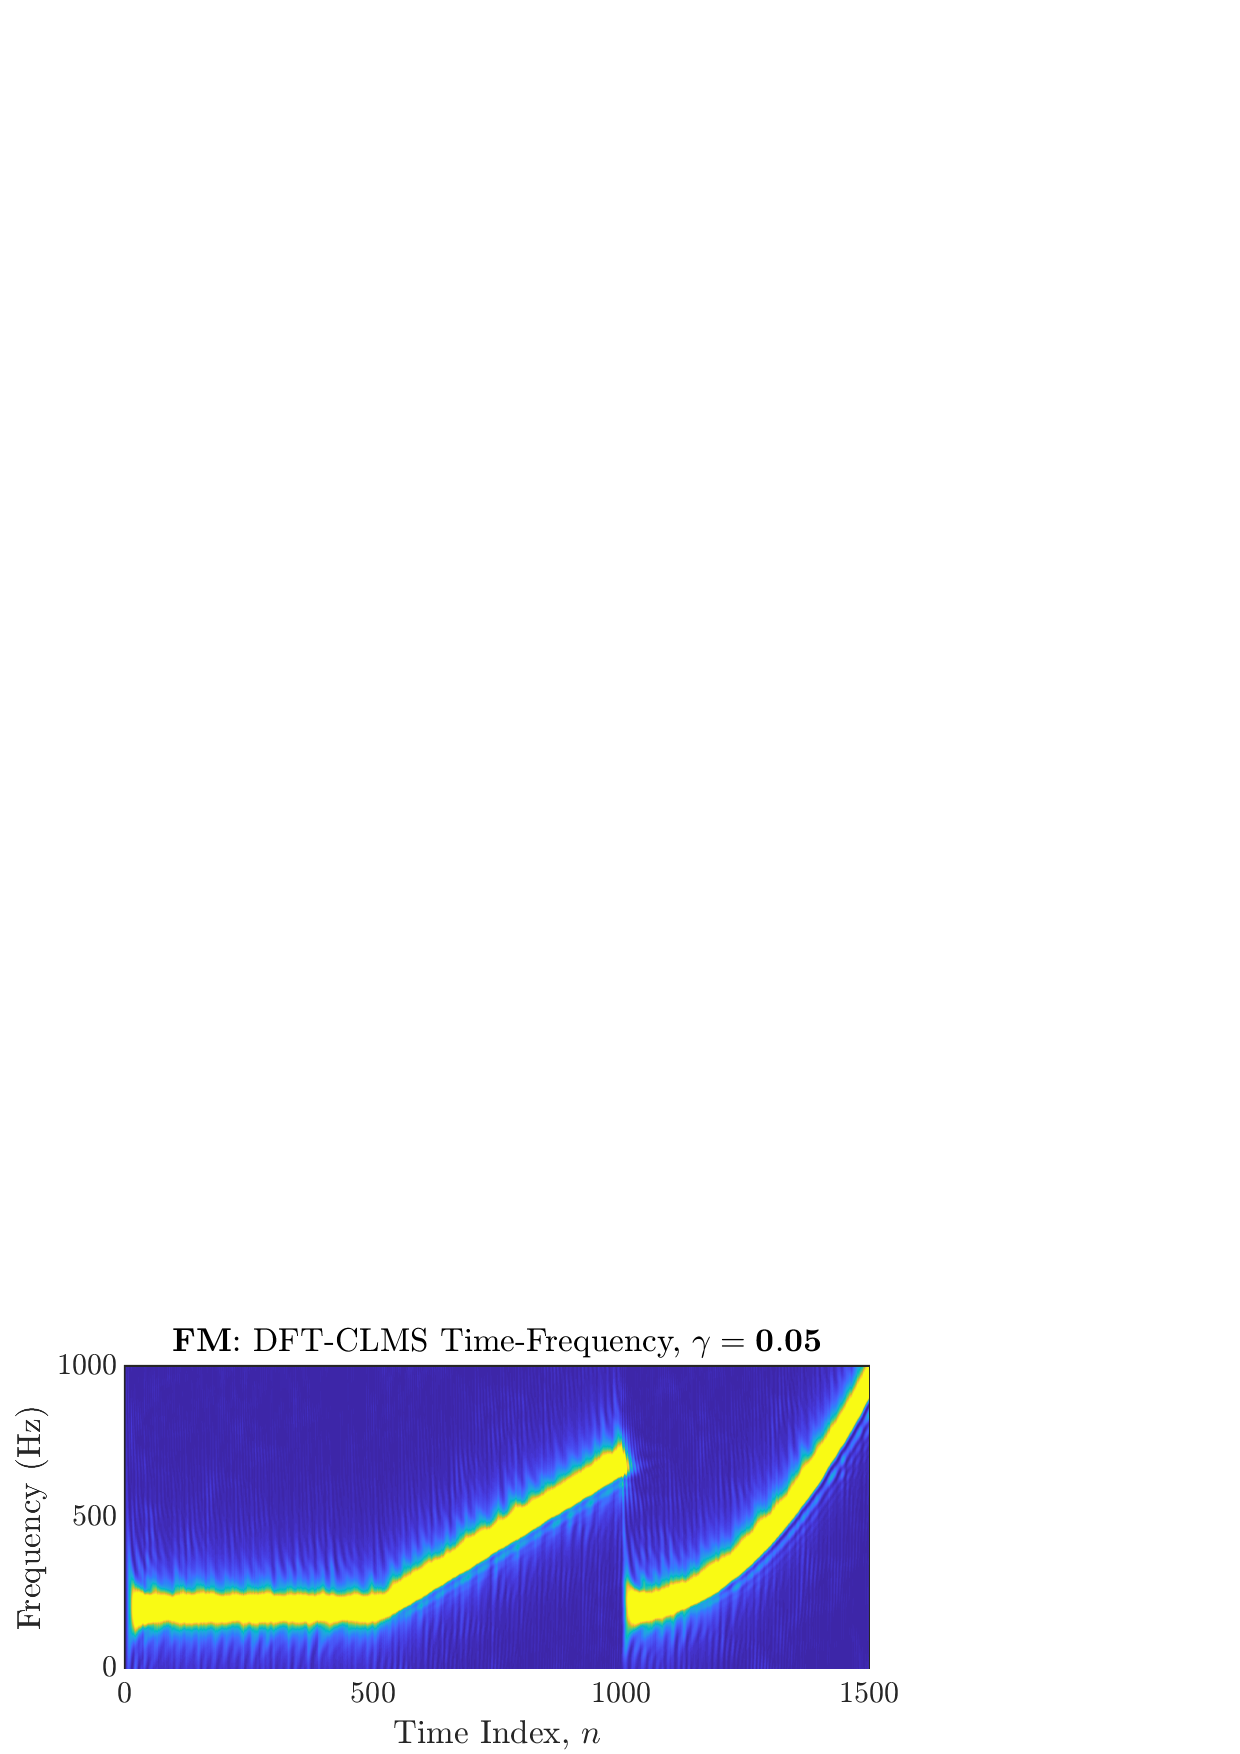
\includegraphics[height=1.5in]{{report/widely-linear-filtering-and-adaptive-spectrum-estimation/a-real-time-spectrum-analyser-using-least-mean-square/assets/c/dft_clms-gamma_0.05}.pdf}
    \end{subfigure}
    ~
    ~
    \begin{subfigure}{0.49\textwidth}
        \centering
        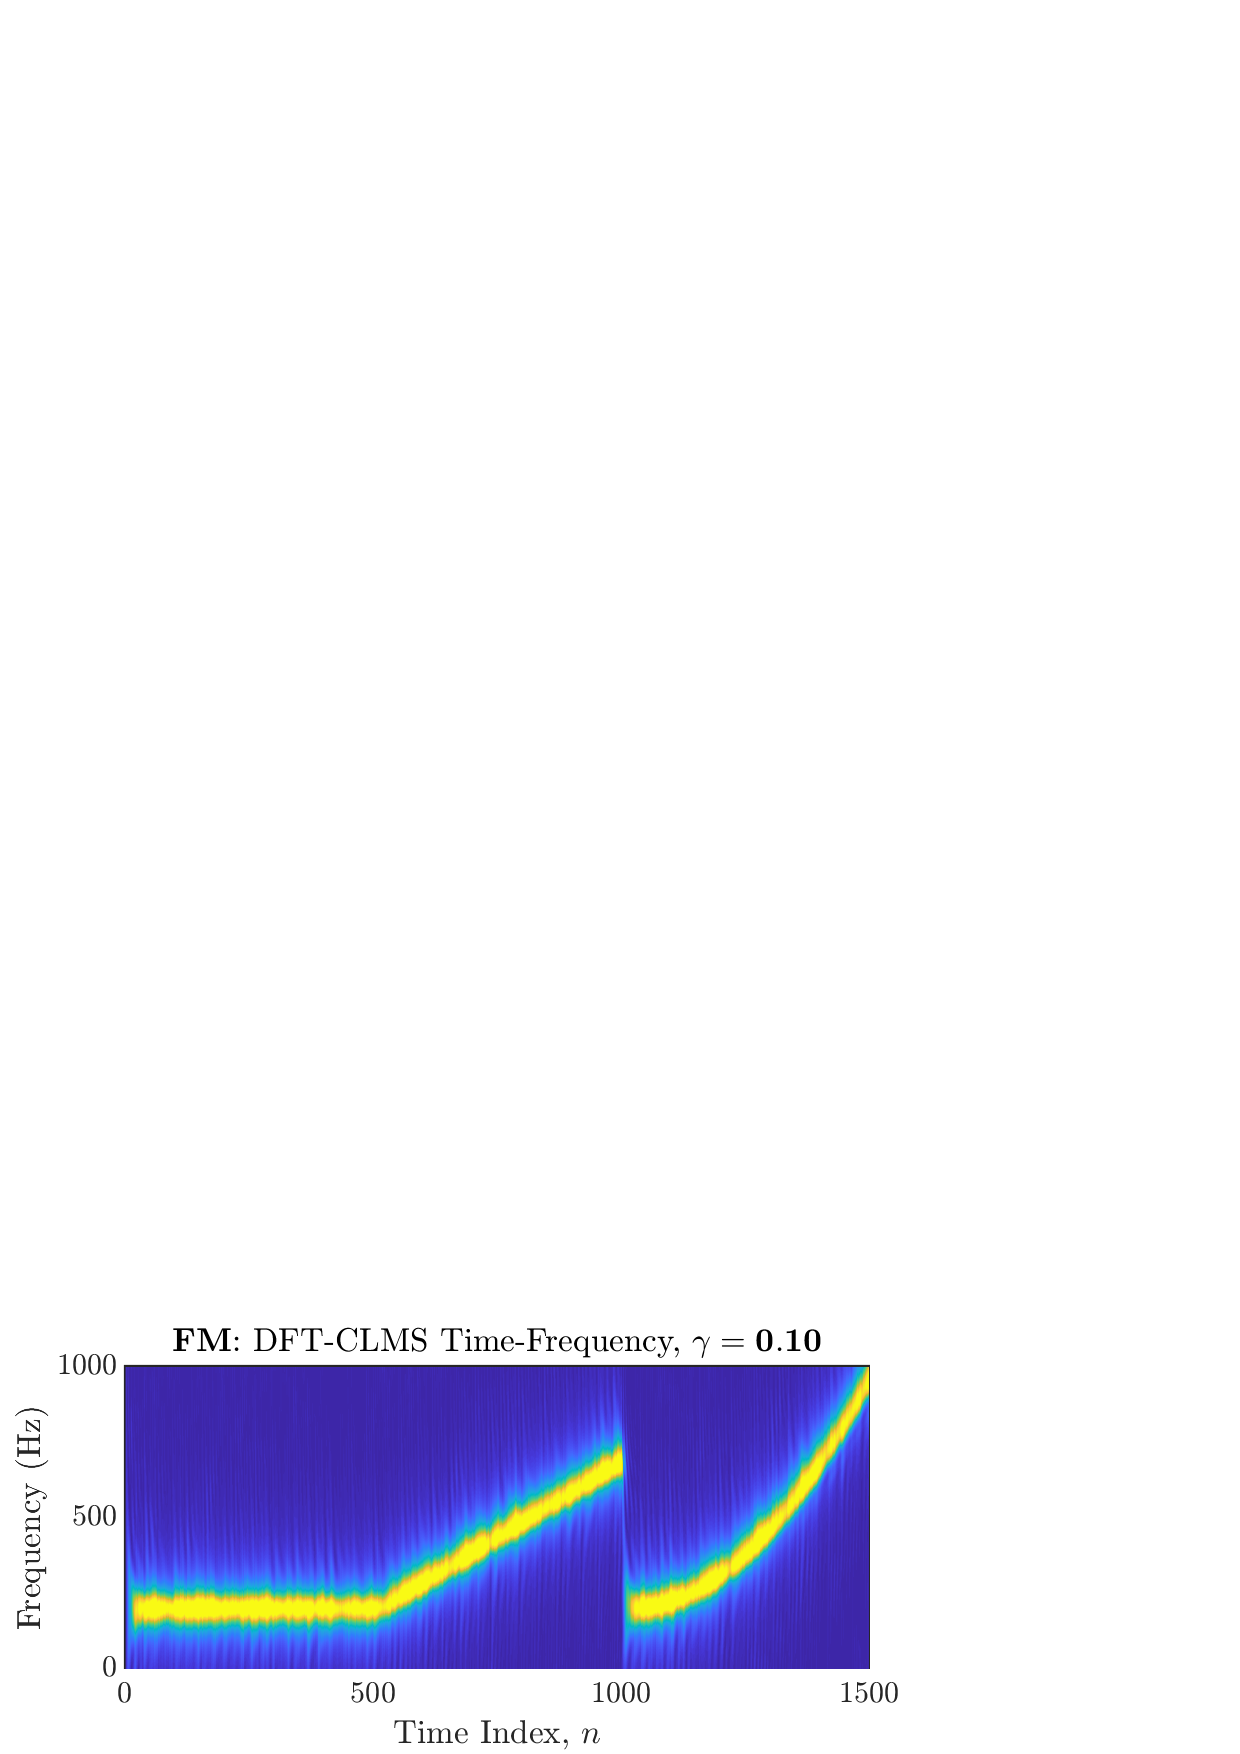
\includegraphics[height=1.5in]{{report/widely-linear-filtering-and-adaptive-spectrum-estimation/a-real-time-spectrum-analyser-using-least-mean-square/assets/c/dft_clms-gamma_0.10}.pdf}
    \end{subfigure}
    ~
    \begin{subfigure}{0.49\textwidth}
        \centering
        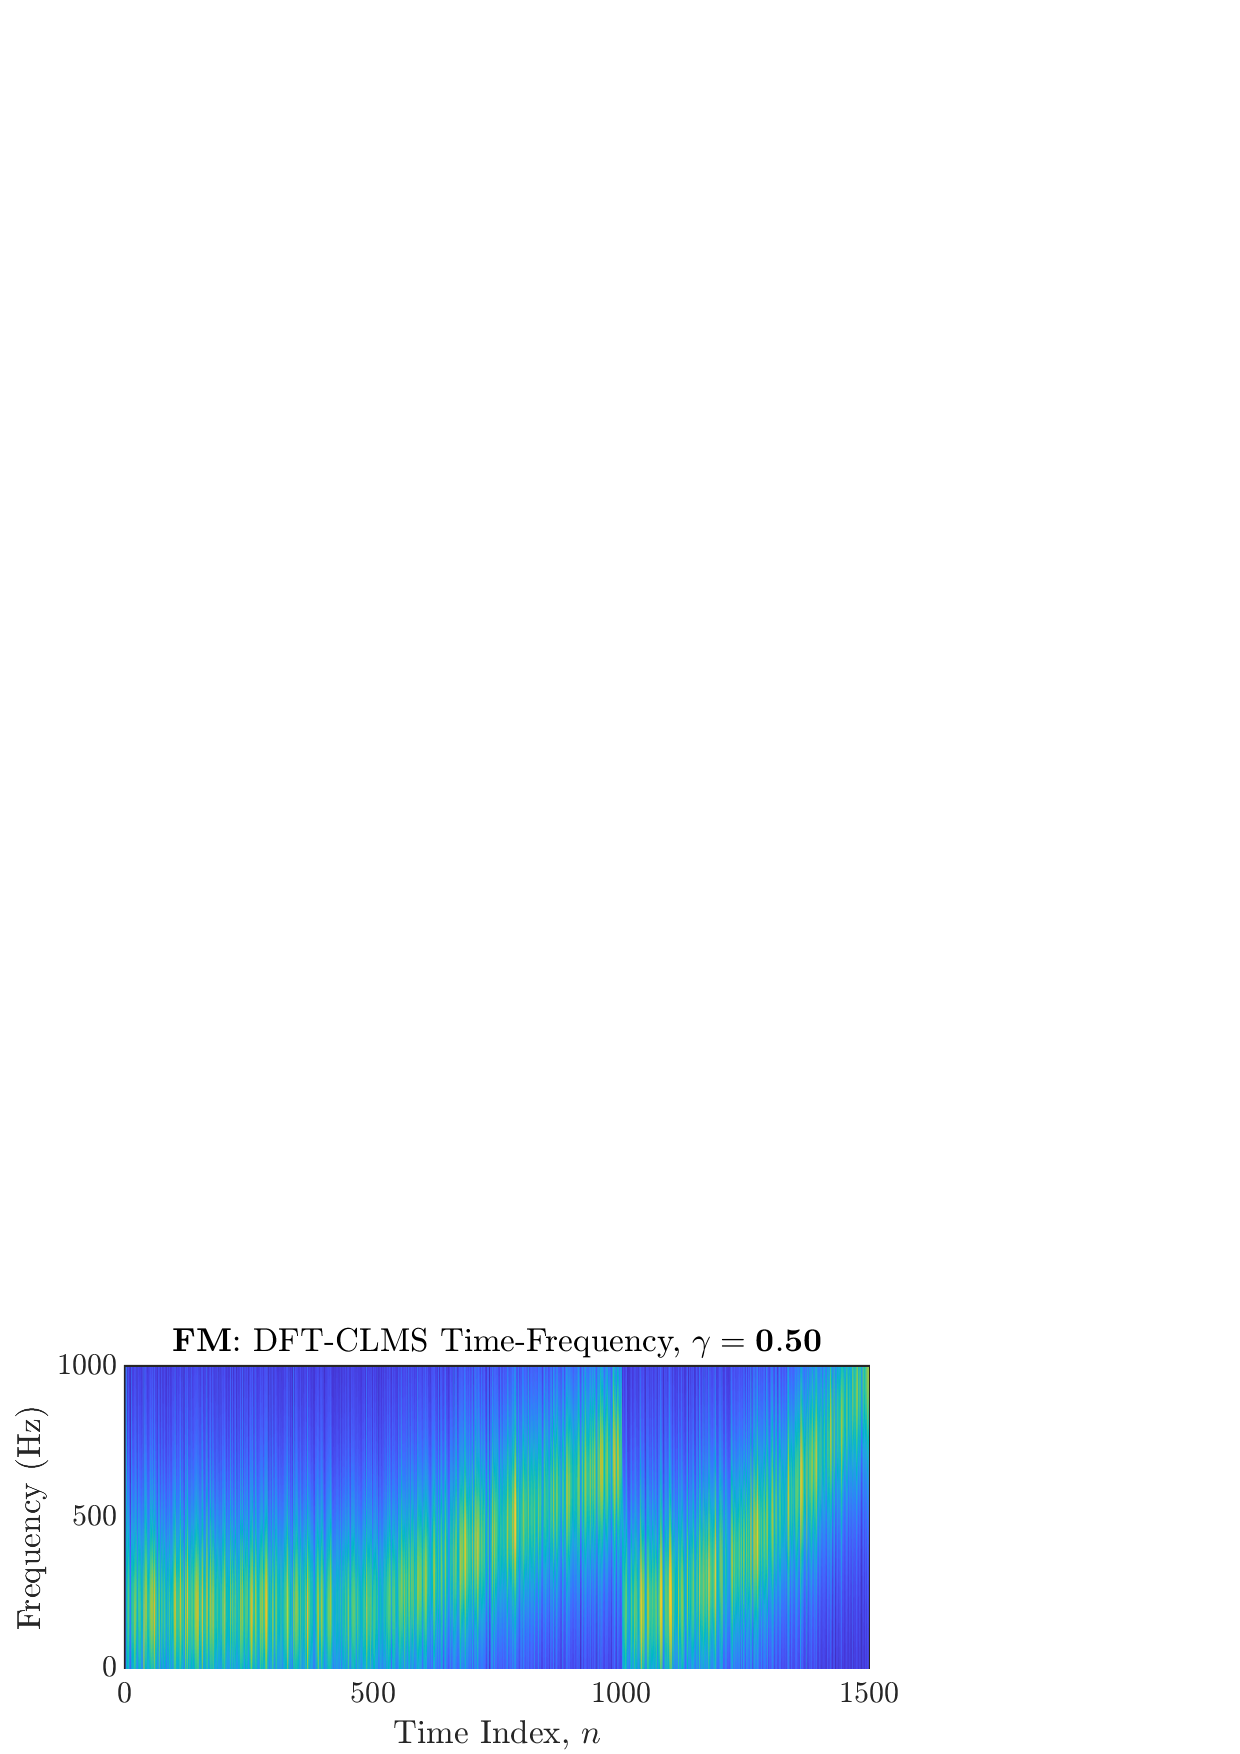
\includegraphics[height=1.5in]{{report/widely-linear-filtering-and-adaptive-spectrum-estimation/a-real-time-spectrum-analyser-using-least-mean-square/assets/c/dft_clms-gamma_0.50}.pdf}
    \end{subfigure}
    \caption{FM: DFT-CLMS time-frequency plot with $\gamma > 0$ (biased).}
    \label{fig:4_3_c_2}
\end{figure}

%% d)
\item
%

The $K$-points DFT-CLMS algorithm is applied to the EEG \texttt{POz} data, of length $N=1200$.
The time-frequency diagrams for different $\gamma$ values are obtained and illustrated in figure \ref{fig:4_3_d}.
The Leaky CLMS does not perform any better than the standard CLMS algorithm, due to the stationary nature of the signal
under study.

\begin{figure}[h]
    \centering
    \begin{subfigure}{0.49\textwidth}
        \centering
        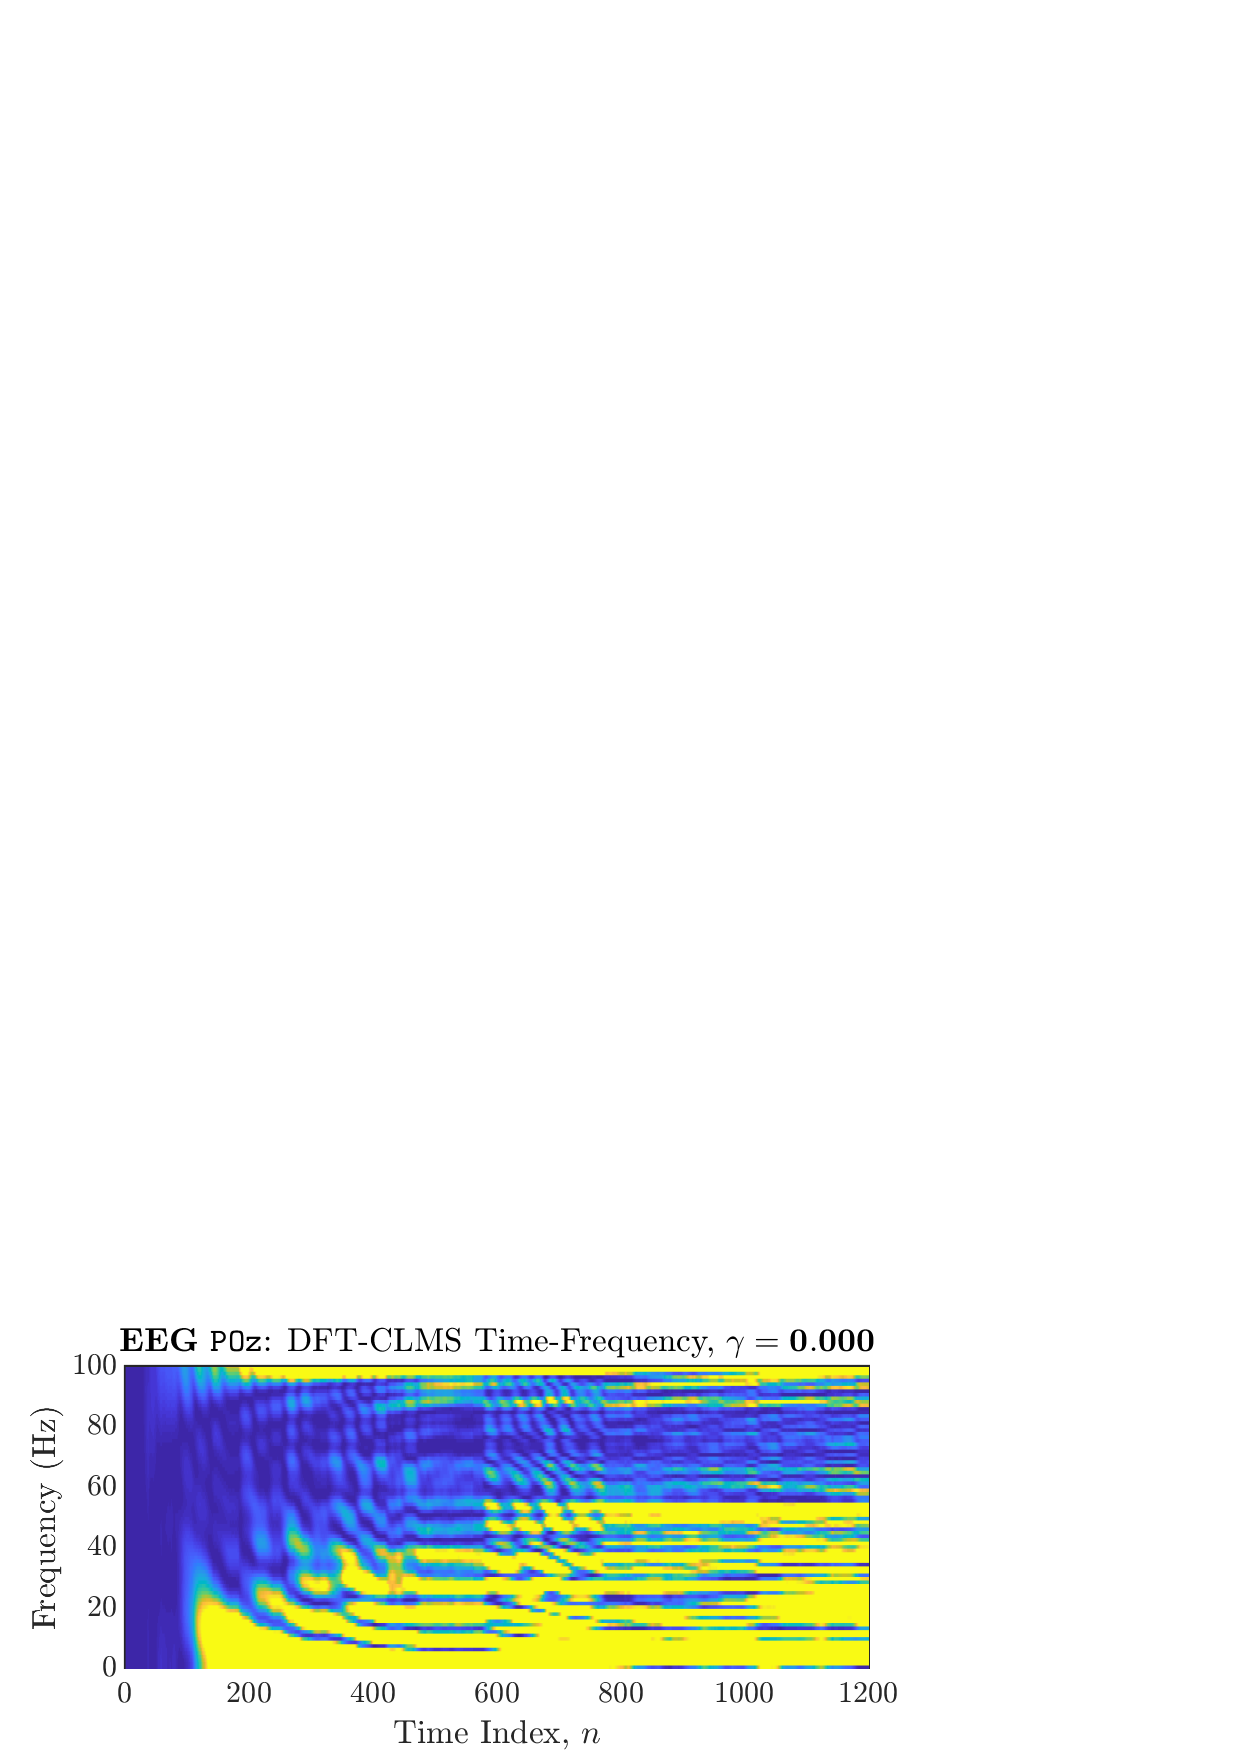
\includegraphics[height=1.5in]{{report/widely-linear-filtering-and-adaptive-spectrum-estimation/a-real-time-spectrum-analyser-using-least-mean-square/assets/d/dft_clms-gamma_0.000}.pdf}
    \end{subfigure}
    ~
    \begin{subfigure}{0.49\textwidth}
        \centering
        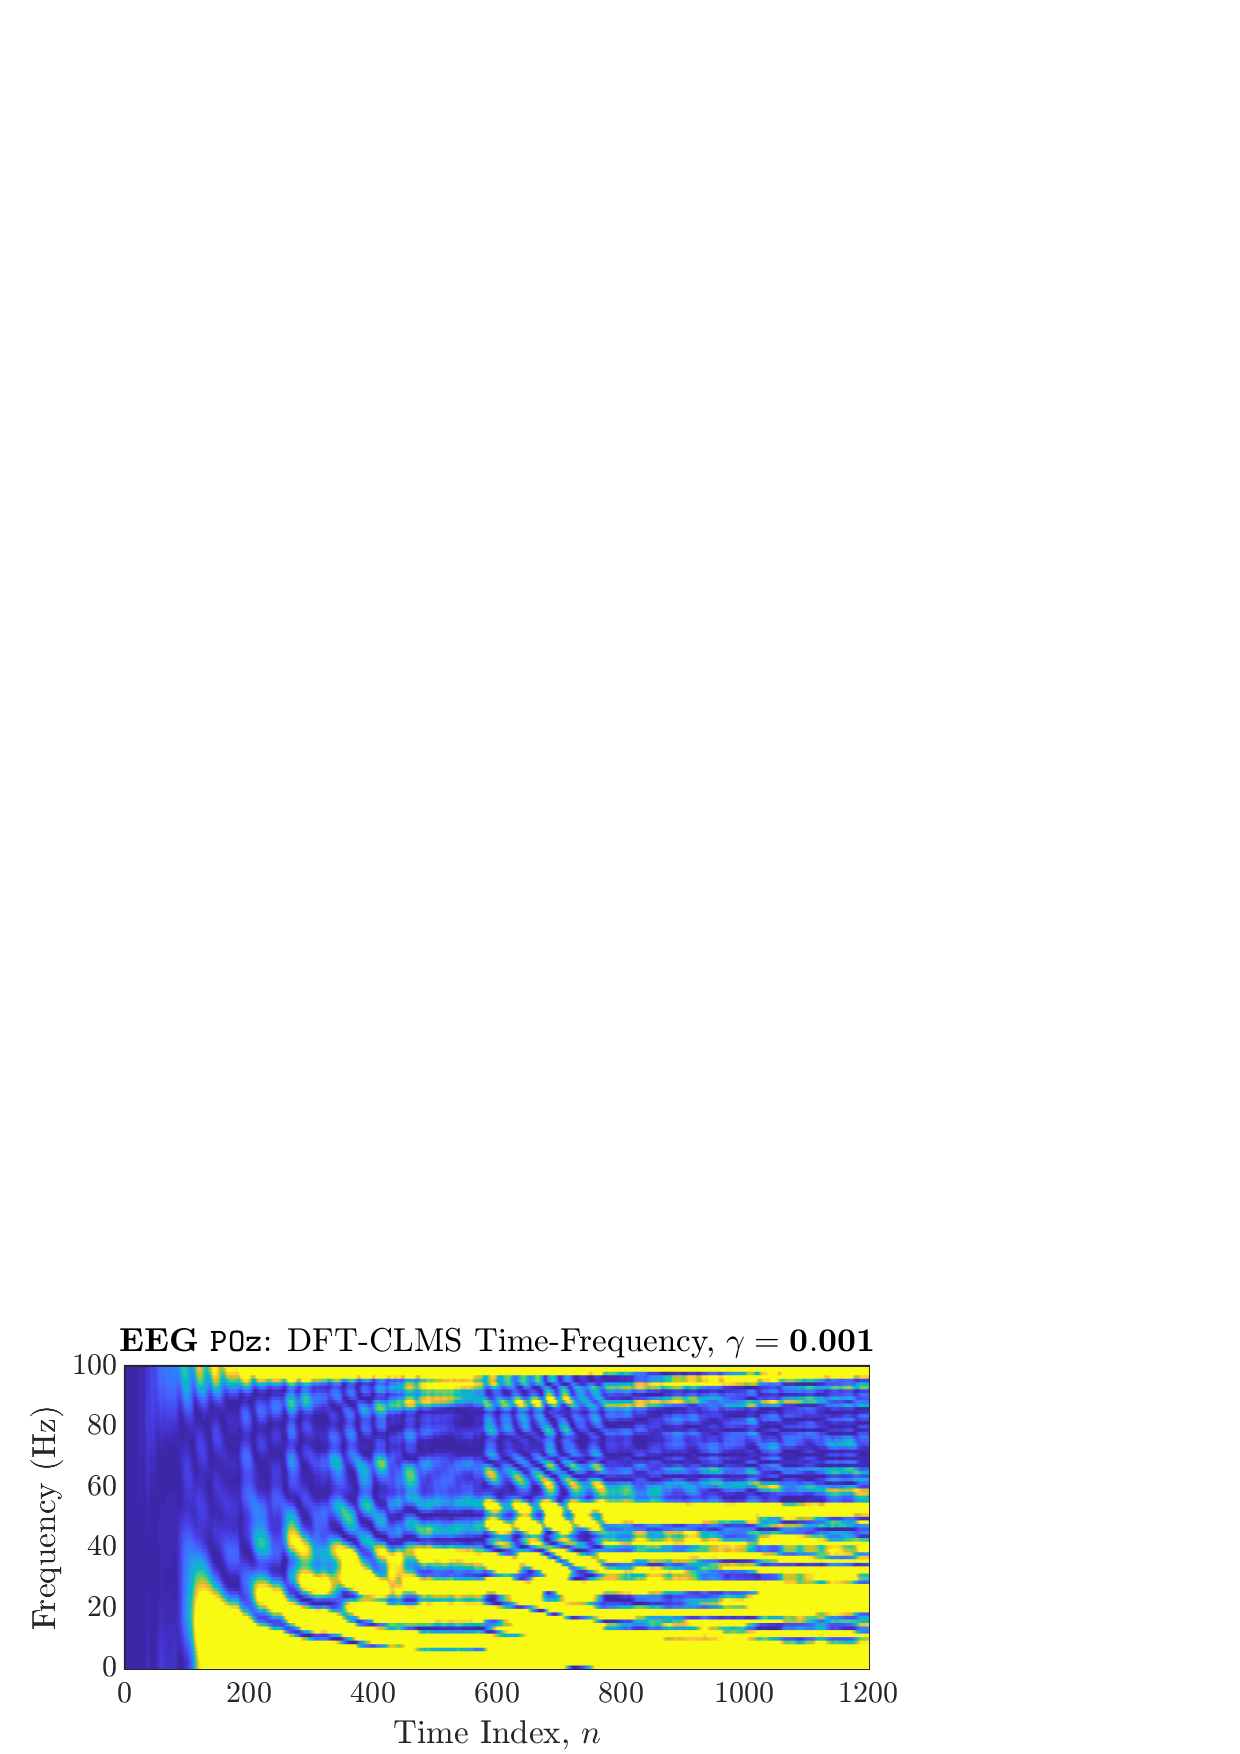
\includegraphics[height=1.5in]{{report/widely-linear-filtering-and-adaptive-spectrum-estimation/a-real-time-spectrum-analyser-using-least-mean-square/assets/d/dft_clms-gamma_0.001}.pdf}
    \end{subfigure}
    \caption{EEG \texttt{POz}: DFT-CLMS time-frequency plots.}
    \label{fig:4_3_d}
\end{figure}

The strong $50 Hz$ component is visible in both implementations and so are the first two harmonics of SSEVP, at
frequencies $f_{1} = 13 Hz$ and $f_{2} = 26 Hz$, respectively. The third harmonic is not distinguishable though, with any
of the two algorithms.

%
\end{enumerate}